% Graph 1 nach "Idee" 
\begin{tikzpicture}[domain=0.5:2,prefix=plots/, smooth]
\draw[very thin,color=gray] (-0.3,0.0) grid (2.5,2.0);
\draw[->] (-0.3,0) -- (2.5,0) node[right] {$x$};
\draw[->] (0,-0.3) -- (0,2) node[above] {$y$};
\draw (0.5,0) node[anchor=north] {$a$};
\draw (2,0) node[anchor=north] {$b$};
\draw[color=blue] plot[id=22.1_int1] function{sin(x)} node[below, midway] {};
\end{tikzpicture}\\*

% Graph 2 vor "Dann zählen flächen"
\begin{tikzpicture}[domain=0.5:2,prefix=plots/, smooth]
\draw[very thin,color=gray] (-0.3,0.0) grid (2.5,2.0);
\draw[->] (-0.3,0) -- (2.5,0) node[right] {$x$};
\draw[->] (0,-0.3) -- (0,2) node[above] {$y$};
\draw (0.5,0) node[anchor=north] {$a$};
\draw (2,0) node[anchor=north] {$b$};
% Label zwischen Graph und X-Achse einfügen
\draw[color=blue] plot[id=22.2_int2] function{sin(2x + 0.5)} node[below, midway] {};
\end{tikzpicture}\\*

%Graph 3 kurz vor 9.1.2
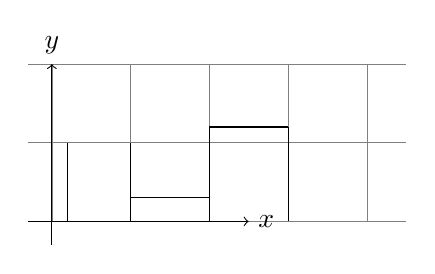
\begin{tikzpicture}
\draw[very thin,color=gray] (-0.3,0.0) grid (4.5,2.0);
\draw[->] (-0.3,0) -- (2.5,0) node[right] {$x$};
\draw[->] (0,-0.3) -- (0,2) node[above] {$y$};
% Schrafierung einfügen
\draw (0.2, 1) -- (0.2, 1);
\draw (0.2, 0) - - (0.2, 1);
\draw (1, 0) - - (1, 1);
\draw (1, 0.3) -- (2, 0.3);
\draw (2, 0) - - (2, 1.2);
\draw (2, 1.2) -- (3, 1.2);
\draw (3, 0) - - (3, 1.2);
\end{tikzpicture}\\*

% Graph 4 nach "BSP"
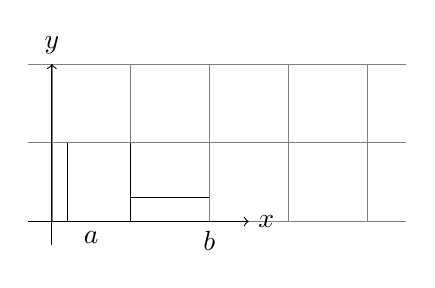
\begin{tikzpicture}
\draw[very thin,color=gray] (-0.3,0.0) grid (4.5,2.0);
\draw[->] (-0.3,0) -- (2.5,0) node[right] {$x$};
\draw[->] (0,-0.3) -- (0,2) node[above] {$y$};
\draw (0.5,0) node[anchor=north] {$a$};
\draw (2,0) node[anchor=north] {$b$};
% Schrafierung einfügen
\draw (0.2, 1) -- (0.2, 1);
\draw (0.2, 0) - - (0.2, 1);
\draw (1, 0) - - (1, 1);
\draw (1, 0.3) -- (2, 0.3);
\end{tikzpicture}\\*

\uS{Das Riemannsche Integral}
\ul{Idee} Sei $f: [a, b] \to \R$ beliebige Funktion.\\*
Wenn $g \leq f$ und $g$ Treppenfunktion dann sollte $\int g(x)dx < \int f(x)dx$
Wenn $f \leq h$ und $f$ Treppenfunktion dann sollte $\int f(x)dx < \int h(x)dx$
Wenn $\int^b_a f(x)dx$ durch diese ($\infty$-vielen) Bedingungen festgelegt wird, nennen wir $f$ integrierbar und $\int_a^b f(x) dx$ ist definiert.

%Stefan

\sS{Bemerkung}
$f:[a,b] \to \R$ ist integrierbar \equ{} es gilt: Für jedes \e > 0 gibt es eine Treppenfunktion $g,\ h$ mit $g \leq f \leq h$ mit $\int_a^b h(x)dx - \int_a^b g(x)dx < \e$. Damit ist $\int_a^b f(x)$ bist auf $\e$ festgelegt.

\sS{Satz Eigenschaften des Integrals}
Seien $f, g: [a, b] \to \R$ integrierbar, dann sind auch $f + g$ und $c \cdot f$ integrierbar und
\enum{
\item $\int_a^b (f + g)(x) dx = \int_a^b f(x) + \int_a^b g(x)$
\item $\int_a^b (c \cdot f)(x) dx = c \cdot \int_a^b f(x)$
\item wenn $f \leq g$ dann $\int f(x)dx \leq \int g(x)dx$
}
\bew
\notat $I(f) = \int f(x)dx$\\*
Sei $\e > 0$ gegeben.\\*
Wähle Treppenfunktion $f_1, f_2, g_1, g_2$ mit $f_1 < f < f_2$ und $g_1 < g < g_2$\\*
$I(f_2) - I(f_1) < \e$, $I(g_2) - I(g_1) < \e$\\*
\Larr{} $f_1 + g_1 < f + g < f_2 + g_2$\\*
%Lustige Pfeile

$I(f_2 + g_2) - I(f_1 + g_1) = I(f_2) - I(f_1) + I(g_2) - I(g_1) < \e + \e = 2\e$\\*
Das für jedes $\e > 0$ \\*
$|I(f + g) - I(f) - I(g)| \leq |I(f + g) - I(f_1 + g_1)| + |I(f) - I(f_1)| + |I(f) - I(f_1)| = 2\e + \e + \e = 4\e$\\*
(Dreiecksungleichung)\\*
\Rarr{} $I(f + g) - I(f) - I(g) = 0$\\
Rest des Satzes analog. \qed{}

% Stefan

% Graph 5
\begin{tikzpicture}[domain=0.5:2,prefix=plots/, samples=10]
\draw[very thin,color=gray] (-0.3,0.0) grid (2.5,2.0);
\draw[->] (-0.3,0) -- (2.5,0) node[right] {$x$};
\draw[->] (0,-0.3) -- (0,2) node[above] {$y$};
\draw[color=blue] plot[id=22.5_x3const, const plot] function{-(x-2)**3} node[below, midway] {};
\draw[color=red] plot[id=22.5_x3] function{-(x-2)**3} node[below, midway] {};
\end{tikzpicture}\\*

% Graph 6
\begin{tikzpicture}[domain=0.5:2,prefix=plots/, smooth]
\draw[very thin,color=gray] (-0.3,0.0) grid (2.5,2.0);
\draw[->] (-0.3,0) -- (2.5,0) node[right] {$x$};
\draw[->] (0,-0.3) -- (0,2) node[above] {$y$};
\draw[color=blue] plot[id=22.6_x3const, const plot, samples=10] function{(0.3x-2)**2} node[below, midway] {};
\draw[color=red] plot[id=22.6_x3] function{(0.3x-2)**2} node[below, midway] {};
\end{tikzpicture}\\*

Zeige \enum{
\item Gegeben sei $\e > 0$\\
6.24 \Rarr{} $f$ gleichmäßig aber stetig. d.h. es gibt $\d > 0$ so dass gilt:\\*
Wenn $|x-y|<\d$ dann $|f(x) - f(y)|<\e$\\*
Wähle Unterteilung $a = x_0 < x_1 < x_2 < ... < x_n = b$ mit $x_i - x_{i-1} < \d$
%Graph
Sei $c := f(x_i)$ \\*
Definiere Treppenfunktion $g:[a,b] \to \R$\\*
$x_{i-1} < x < x_i$ \Rarr{} $g(x) = c_i = f(x)\ (1 \leq i \leq n)$\\*
$g(x_0) = f(x_0)$ dann $|f(x) - g(x)| < \e$ für alle $x$.\qed{}
}

\Rarr{} $f(x_1)(b-a) = \int_a^b f(x) \leq \int_a^b dx \leq_a^bf(x_2) dx = f(x_2)(b-a)$\\*
$f(x_1) \leq \frac{1}{b-a} \int_a^b f(x)dx \leq f(x)$\\*
Zwischenwertsatz \Rarr{} es gibt auch $x_0 \in [a, b]$ mit $f(x_0) = y$ \Rarr{} $f(x_0)(b-a) = \int_a^b f(x)dx$